\section{Date: 2026-08-23}
\noindent \textbf{Series ID: EDEF} 

\noindent This series is titled Equipment Deflator and has a frequency of Quarterly. The units are Index 2017=100 and the seasonal adjustment is Seasonally Adjusted.The observation start date is 1947-01-01 and the observation end date is 2024-10-01.The popularity of this series is 3. \\ 

\noindent \textbf{Series ID: KOREPUINDXM} 

\noindent This series is titled Economic Policy Uncertainty Index for South Korea (DISCONTINUED) and has a frequency of Monthly. The units are Index and the seasonal adjustment is Not Seasonally Adjusted.The observation start date is 1990-01-01 and the observation end date is 2014-12-01.The popularity of this series is 5. \\ 

\subsection{Raw Regression}
\noindent Regresses the two series against each other directly. A significant result here can come just as easily from both series sharing a long-run trend as from any real relationship.

\begin{center}
\begin{tabular}{lclc}
\toprule
\textbf{Dep. Variable:}    & value\_fred\_KOREPUINDXM & \textbf{  R-squared:         } &     0.272   \\
\textbf{Model:}            &           OLS            & \textbf{  Adj. R-squared:    } &     0.264   \\
\textbf{Method:}           &      Least Squares       & \textbf{  F-statistic:       } &     36.53   \\
\textbf{Date:}             &     Sun, 23 Aug 2026     & \textbf{  Prob (F-statistic):} &  2.72e-08   \\
\textbf{Time:}             &         12:14:53         & \textbf{  Log-Likelihood:    } &   -510.09   \\
\textbf{No. Observations:} &             100          & \textbf{  AIC:               } &     1024.   \\
\textbf{Df Residuals:}     &              98          & \textbf{  BIC:               } &     1029.   \\
\textbf{Df Model:}         &               1          & \textbf{                     } &             \\
\textbf{Covariance Type:}  &        nonrobust         & \textbf{                     } &             \\
\bottomrule
\end{tabular}
\begin{tabular}{lcccccc}
                           & \textbf{coef} & \textbf{std err} & \textbf{t} & \textbf{P$> |$t$|$} & \textbf{[0.025} & \textbf{0.975]}  \\
\midrule
\textbf{const}             &     168.3743  &       12.566     &    13.399  &         0.000        &      143.437    &      193.311     \\
\textbf{value\_fred\_EDEF} &      -0.3560  &        0.059     &    -6.044  &         0.000        &       -0.473    &       -0.239     \\
\bottomrule
\end{tabular}
\begin{tabular}{lclc}
\textbf{Omnibus:}       & 14.723 & \textbf{  Durbin-Watson:     } &    1.266  \\
\textbf{Prob(Omnibus):} &  0.001 & \textbf{  Jarque-Bera (JB):  } &   16.725  \\
\textbf{Skew:}          &  0.843 & \textbf{  Prob(JB):          } & 0.000233  \\
\textbf{Kurtosis:}      &  4.083 & \textbf{  Cond. No.          } &     668.  \\
\bottomrule
\end{tabular}
%\caption{OLS Regression Results}
\end{center}

Notes: \newline
 [1] Standard Errors assume that the covariance matrix of the errors is correctly specified.

\begin{figure}
\centering
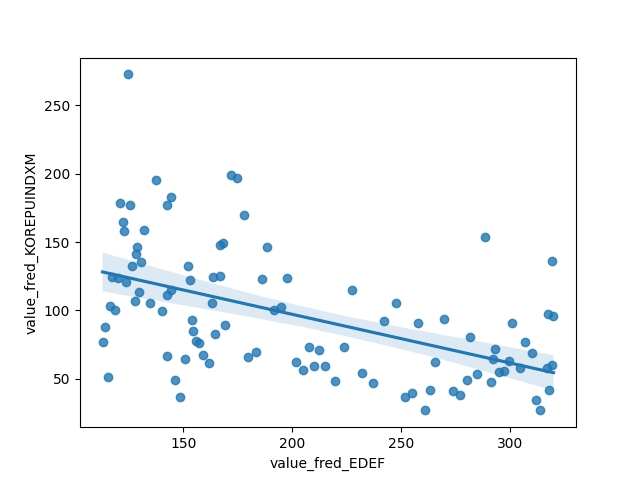
\includegraphics[scale = 0.9]{plots/plot_2026-08-23.png}
\caption{Raw Regression Plot for 2026-08-23}
\end{figure}
\newpage
\subsection{Detrended Regression}
\noindent Regresses the residuals of each series after removing its own linear time trend, so a shared trend can no longer drive the result on its own. A relationship that stays significant here is better evidence of a genuine link between the two series.

\begin{center}
\begin{tabular}{lclc}
\toprule
\textbf{Dep. Variable:}               & value\_fred\_KOREPUINDXM\_detrended & \textbf{  R-squared:         } &     0.013   \\
\textbf{Model:}                       &                 OLS                 & \textbf{  Adj. R-squared:    } &     0.002   \\
\textbf{Method:}                      &            Least Squares            & \textbf{  F-statistic:       } &     1.246   \\
\textbf{Date:}                        &           Sun, 23 Aug 2026          & \textbf{  Prob (F-statistic):} &    0.267    \\
\textbf{Time:}                        &               12:14:54              & \textbf{  Log-Likelihood:    } &   -510.09   \\
\textbf{No. Observations:}            &                   100               & \textbf{  AIC:               } &     1024.   \\
\textbf{Df Residuals:}                &                    98               & \textbf{  BIC:               } &     1029.   \\
\textbf{Df Model:}                    &                     1               & \textbf{                     } &             \\
\textbf{Covariance Type:}             &              nonrobust              & \textbf{                     } &             \\
\bottomrule
\end{tabular}
\begin{tabular}{lcccccc}
                                      & \textbf{coef} & \textbf{std err} & \textbf{t} & \textbf{P$> |$t$|$} & \textbf{[0.025} & \textbf{0.975]}  \\
\midrule
\textbf{const}                        &    1.011e-11  &        4.013     &  2.52e-12  &         1.000        &       -7.963    &        7.963     \\
\textbf{value\_fred\_EDEF\_detrended} &      -0.3415  &        0.306     &    -1.116  &         0.267        &       -0.949    &        0.266     \\
\bottomrule
\end{tabular}
\begin{tabular}{lclc}
\textbf{Omnibus:}       & 14.693 & \textbf{  Durbin-Watson:     } &    1.266  \\
\textbf{Prob(Omnibus):} &  0.001 & \textbf{  Jarque-Bera (JB):  } &   16.673  \\
\textbf{Skew:}          &  0.842 & \textbf{  Prob(JB):          } & 0.000240  \\
\textbf{Kurtosis:}      &  4.079 & \textbf{  Cond. No.          } &     13.1  \\
\bottomrule
\end{tabular}
%\caption{OLS Regression Results}
\end{center}

Notes: \newline
 [1] Standard Errors assume that the covariance matrix of the errors is correctly specified.

\begin{figure}
\centering
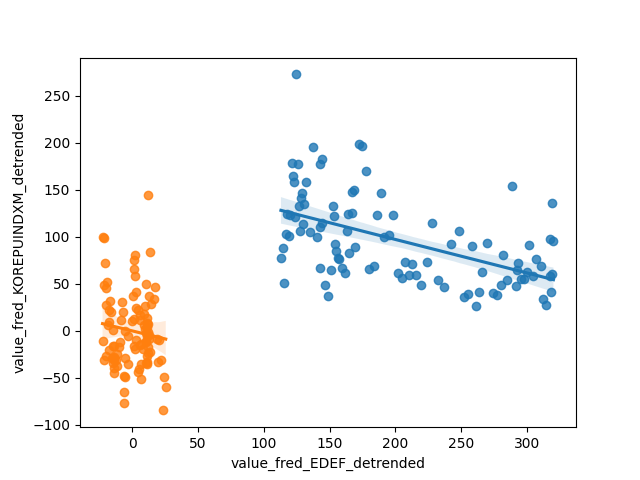
\includegraphics[scale = 0.9]{plots/plot_2026-08-23_detrended.png}
\caption{Detrended Regression Plot for 2026-08-23}
\end{figure}
\newpage
